\chapter{Divide and Conquer}
\label{ch:design::dc}

\begin{preamble}
This chapter describes the divide-and-conquer technique, an important algorithm-design technique, and applies it to several problems.
%
Divide and conquer is an effective technique for solving a variety of problems, and usually leads to efficient and parallel algorithms.
%
\end{preamble}

\section{Divide and Conquer}
\label{sec:design::dc}

\begin{gram}

A divide-and-conquer algorithm has a distinctive anatomy: it has a base case to handle small instances and an inductive step with three
distinct phases: ``divide'', ``recur'', and ``combine.''
%
The \defn{divide}~phase divides the problem instance into smaller instances;
%
the \defn{recur}~phase solves the smaller instances;
%
and the \defn{combine} phase combines the results for the smaller
instance to construct the result to the larger instance.
%
\end{gram}

\begin{flex}
\begin{definition}[Divide-And-Conquer Algorithm]
A divide-and-conquer algorithm has the following structure.
%
\begin{description}
\item[Base Case:] When the instance $I$ of the problem $P$ is
  sufficiently small, compute the solution $P(I)$ perhaps by using a
  different algorithm.

\item[Inductive Step:]\mbox{}
\begin{enumerate}
\item {\bf Divide} instance $I$ into some number of 
smaller instances of the same problem $P$.
\item {\bf Recur} on each of the smaller instances and compute
  their solutions.
\item {\bf Combine} the solutions to obtain the solution to the
  original instance $I$.
\end{enumerate}
\end{description}
\end{definition}

%% \begin{comment}
%% Note that CLRS when defining DandC refers to the instance as a
%% ``problem'' and sub instances as ``subproblems''.  This is
%% inconsistent with their previous definition of ``problem'' meaning the
%% general problem, and ``instance'' meaning a particular instance.  Lets
%% avoid falling into the same trap.
%% \end{comment}

\begin{example}
The drawing below illustrates the structure of a divide-and-conquer
algorithm that divides the problem instance into three independent
subinstances.

\begin{center}
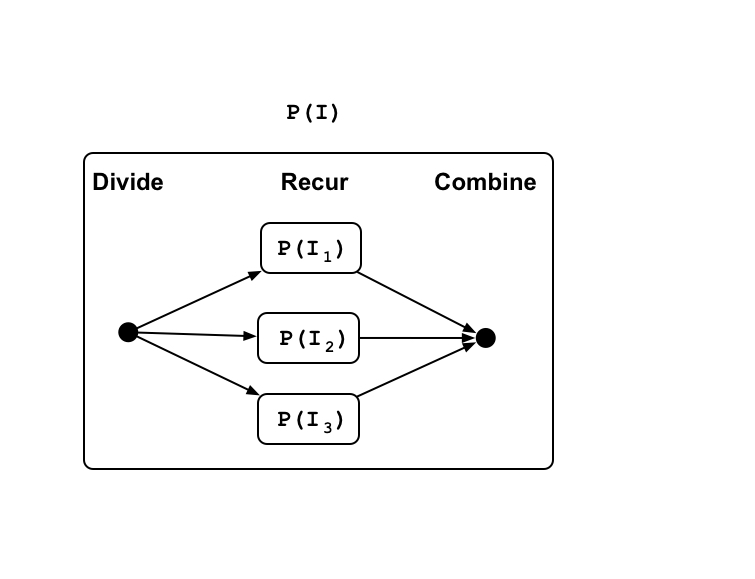
\includegraphics[width=5in]{./design/media-dc/divide-and-conquer.jpg}
\end{center}
\end{example}
\end{flex}

\begin{gram}[Properties of Divide-and-Conquer Algorithms]
Divide-and-Conquer has several important properties.  
%

\begin{itemize}
\item  It follows the structure of an inductive proof, and therefore
usually leads to relatively simple proofs of correctness. 
%
To prove a divide-and-conquer algorithm correct, we first prove that the
base case is correct.  Then, we assume by strong (or structural)
induction that the recursive solutions are correct, and show that,
given correct solutions to smaller instances, the combined solution is
correct.
%

\item Divide-and-conquer algorithms can be work efficient.
%
To ensure efficiency, we need to make sure that the divide and combine
steps are efficient, and that they do not create too many
sub-instances.
%

\item The work and span for a divide-and-conquer algorithm can be
  expressed as a mathematical equation called \href{ch:analysis::recurrences}{recurrence},
which can be usually be solved without too much difficulty.
%

\item Divide-and-conquer algorithms are naturally parallel, because
  the sub-instances can be solved in parallel.  This can lead to
  significant amount of parallelism, because each inductive step can
  create more independent instances. For example, even if the
  algorithm divides the problem instance into two subinstances, each
  of those subinstances could themselves generate two more
  subinstances, leading to a geometric progression, which can quickly
  produce abundant parallelism.
\end{itemize}
\end{gram}

\begin{gram}[Analysis of Divide-and-Conquer Algorithms]
Consider an algorithm that divides a problem instance of size $n$ into
$k > 1$ independent subinstances of sizes $n_1, n_2, \ldots n_k$,
recursively solves the instances, and combine the solutions to
construct the solution to the original instance.

We can write the work of such an algorithm using the recurrence then
\begin{align*}
  W(n) \;&=\; W_{\textrm{divide}}(n) \;+\; \sum_{i=1}^k W(n_i) \;+\; W_{\textrm{combine}}(n) + 1.
\end{align*}
%
The work recurrence simply adds up the work across all phases of the
algorithm (divide, recur, and combine).

To analyze the span, note that after the instance is divided into
subinstance, the subinstances can be solved in parallel (because they
are independent), and the results can be combined.  The span can thus
be written as the recurrence:
%
\begin{align*}
S(n) &= S_{\textrm{divide}}(n) \;+\; \max_{i=1}^k S(n_i) \;+\; S_{\textrm{combine}}(n) + 1.\\
\end{align*}
\end{gram}

\begin{note}
The work and span recurrences for a divide-and-conquer algorithm
usually follow the recursive structure of the algorithm, but is a
function of size of the arguments instead of the actual values.
\end{note}


\begin{example}[Maximal Element]
We can find the maximal element in a sequence using divide and conquer
as follows.
%
If the sequence has only one element, we return that element,
otherwise, we divide the sequence into two equal halves and
recursively and in parallel compute the maximal element in each half.
%
We then return the maximal of the results from the two recursive
calls.
%
For a sequence of length $n$, we can write the work and span for this
algorithm as recurrences as follows:
\[
W(n) = \left\{
\begin{array}{lll}
\Theta(1) & \mbox{if} & n \le 1
\\
2W(n/2) + \Theta(1) &  \mbox{otherwise}
\end{array}
\right.
\]
%
\[
S(n) = \left\{
\begin{array}{lll}
\Theta(1) & \mbox{if} & n \le 1
\\
S(n/2) + \Theta(1) &  \mbox{otherwise}.
\end{array}
\right.
\]
%
This recurrences yield 
\begin{align*}
W(n) & = \Theta(n)~\mbox{and}
\\
S(n) & = \Theta(\lg{n}).
\end{align*}
\end{example}


\begin{algorithm}[Reduce with Divide and Conquer]
\label{alg:design::dc::reduce}
The~\defn{reduce} primitive performs a computation that involves
applying an associative binary operation $op$ to the elements of a
sequence to obtain (reduce the sequence to) a final value.
%
For example, reducing the sequence $\cseq{0,1,2,3,4}$ with the $+$
operation gives us $0 + 1 + 2 + 3 + 4 = 10$.
%
If the operation requires constant work (and thus span), then the work
and span of a reduction is $\Theta(n)$ and $\Theta(\lg{n})$ respectively.

We can write the code for the reduce primitive on sequences as
follows.

\[
\begin{array}{l}
\cdvar{reduceDC}~f~\cdvar{id}~a =
\\
~~~~\cd{if}~\cdvar{isEmpty}~ a~\cd{then}
\\
~~~~~~~~\cdvar{id}
\\
~~~~\cd{else}~\cd{if}~\cdvar{isSingleton}~a~\cd{then}
\\
~~~~~~~~a[0]
\\
~~~~\cd{else}
\\ 
~~~~~~~~\cd{let}
\\ 
~~~~~~~~~~~~(l, r) = \cdvar{splitMid}~a
\\
~~~~~~~~~~~~(a, b) = (\cdvar{reduceDC}~f~\cdvar{id}~l~\cpar{}~\cdvar{reduceDC}~f~\cdvar{id}~r)
\\
~~~~~~~~\cd{in} 
\\
~~~~~~~~~~~~f(a,b)
\\ 
\cd{end}        
\end{array} 
\]
\end{algorithm}

\section{Merge Sort}
\label{sec:design::dc::msort}

\begin{gram}
In this section, we consider the comparison sorting problem and the
merge-sort algorithm, which offers a divide-and-conquer algorithm for
it.
\end{gram}

\begin{definition}[The Comparison-Sorting Problem]
\label{def:problem::comparison-sorting}
  Given a sequence $a$ of elements from a universe $U$, with a total
  ordering given by $<$, return the same elements in a sequence $r$
  in sorted order, i.e. $r[i] \leq r[i+1], 0 < i \leq |a|-1$.
\end{definition}

\begin{algorithm}[Merge Sort]
\label{alg:design::dc::mergesort}

Given an input sequence, merge sort divides it into two sequences that
are approximately half the length, sorts them recursively, and merges
the sorted sequences.
%
Mergesort can be written as follows.

\[
\begin{array}{l}
\cdvar{mergeSort}~a =
\\ 
~~~~\cd{if}~|a| \leq 1~\cd{then}
\\ 
~~~~~~~~a
\\
~~~~\cd{else}
\\ 
~~~~~~~~\cd{let}
\\
~~~~~~~~~~~~(l,r) = \cdvar{splitMid}~a
\\ 
~~~~~~~~~~~~(l',r') = (\cdvar{mergeSort}~l \cpar{} \cdvar{mergeSort}~r)
\\
~~~~~~~~\cd{in}
\\ 
~~~~~~~~~~~~\cdvar{merge} (l',r')
\\
~~~~~~~~\cd{end}
\end{array} 
\]
\end{algorithm}


\begin{note}
In the merge sort algorithm given above the base case is when the
sequence is empty or contains a single element.  In practice, however,
instead of using a single element or empty sequence as the base case,
some implementations use a larger base case consisting of perhaps ten
to twenty keys.
%
\end{note}

\begin{gram}[Correctness and Cost]

To prove correctness we first note that the base case is correct.
Then by induction we note that $l'$ and $r'$ are sorted
versions of $l$ and $r$.
%
Because $l$ and $r$ together contain exactly the same elements as $a$,
we conclude that $\cd{merge}~(l',r')$ returns a sorted version of $a$.


For the work and span analysis, we assume that merging can be done in $\Theta(n)$ work and $\Theta(\lg{n})$ span, where $n$ is the sum of the lengths of the two sequences.
%
We can thus write the work and span for this sorting algorithm
as
\[
W(n) = \left\{
\begin{array}{lll}
\Theta(1) & \mbox{if} & n \le 1
\\
2W(n/2) + \Theta(n) &  \mbox{otherwise}
\end{array}
\right.
\]
%
\[
S(n) = \left\{
\begin{array}{lll}
\Theta(1) & \mbox{if} & n \le 1
\\
S(n/2) + \Theta(\lg{n}) &  \mbox{otherwise}.
\end{array}
\right.
\]

The recurrences solve to
\begin{align*}
W(n) & = \Theta(n\lg{n})
\\
S(n) & = \Theta(\lg^2{n}).
\end{align*}
\end{gram}
%

\begin{remark}[Quick  Sort]
Another divide-and-conquer algorithm for sorting is the quick-sort
algorithm.
% 
Like merge sort, quick sort requires $\Theta(n \log n)$ work, which
is optimal for the comparison sorting problem, but only ``in expectation'' over random decisions that it makes during its execution.
%
While merge sort has a trivial divide step and interesting combine
step, quick sort has an interesting divide step but trivial combine
step.
%
We will study quick sort in greater detail.
%
%\ref{}
\end{remark}

\section{Sequence Scan}
\label{sec:design::dc::scan}

\begin{gram}[Intuition for Scan with Divide and Conquer]
To develop some intuition on how to design a divide-and-conquer
algorithm for the sequence scan problem, let's start by
dividing the sequence in two halves, solving each half, and then
putting the results together. 

For example,  consider the sequence $\cseq{2,1,3,2,2,5,4,1}$.
%
If we divide in the middle and scan over the two resulting sequences
we obtain $(b,b')$ and $(c,c')$, such that 
\begin{align*}
(b, b') & = \left(\cseq{0, 2, 3, 6}, 8 \right),~\mbox{and}
\\
(c, c') & = \left(\cseq{0, 2, 7, 11}, 12\right).
\end{align*}
%

Note now that $b$ already gives us the first half of the solution.
%
To compute the second half, observe that in calculating $c$ in the
second half, we started with the identity instead of the sum of the
first half, $b'$.  
%
Therefore, if we add the sum of the first half, $b'$, to each element
of $c$, we would obtain the desired result.  
%
\end{gram}


\begin{algorithm}[Scan with Divide and Conquer]
By refining the intuitive description above, we can obtain a
divide-and-conquer algorithm for sequences scan, which is given below.

\[
\begin{array}{l}
\cdvar{scanDC}~f~\cdvar{id}~a =
\\
~~~~\cd{if}~|a| = 0~\cd{then}
\\
~~~~~~~~(\cseq{}, \cdvar{id})
\\
~~~~\cd{else if}~|a| = 1~\cd{then}
\\ 
~~~~~~~~(\cseq{\cdvar{id}},a[0])
\\
~~~~\cd{else}
\\ 
~~~~~~~~\cd{let}
\\ 
~~~~~~~~~~~~(b, c) = \cdvar{splitMid}~a
\\
~~~~~~~~~~~~((l,b'),(r,c')) = (\cdvar{scanDC}~f~\cdvar{id}~b \cpar{}~\cdvar{scanDC}~f~\cdvar{id}~c)
\\
~~~~~~~~~~~~r' = \cseq{f (b',x) : x \in r}
\\
~~~~~~~~\cd{in}
\\
~~~~~~~~~~~~(\cdvar{append}~(l,r'), f(b',c'))
\\
~~~~~~~~\cd{end}
\end{array}
\]
\end{algorithm}
%

\begin{remark}
Observe that this algorithm takes advantage of the fact that $\cdvar{id}$ is
really the identity for $f$, i.e. $f(id,x) = x$.
\end{remark}

\begin{gram}[Cost Analysis]
We consider the work and span for the algorithm.  Note that the
combine step requires a map to add $b'$ to each element of $c$, and
then an append.  Both these take $O(n)$ work and $O(1)$ span, where $n
= |a|$.
%
This leads to the following recurrences for the whole
algorithm:
\[
\begin{array}{lllll}
W(n) & = & 2W(n/2) + O(n) & \in &  O(n \log n)
\\
S(n) & = & S(n/2) + O(1) & \in & O(\log n).
\end{array}
\]
Although this is much better than $O(n^2)$ work, we can do better by
using another design technique called contraction.
\end{gram}


\section{Euclidean Traveling Salesperson Problem}
\label{sec:design::dc::etsp}

\begin{gram}
We consider a variant of the  well-known Traveling Salesperson Problem (TSP) and design a divide-and-conquer heuristic for it.
%
%
This variant, known as the Euclidean Traveling Salesperson Problem
(eTSP), is $\textbf{NP}$ hard.
%
It requires solving the TSP problem in graphs where the vertices
(e.g., cities) lie in a Euclidean space and the edge weights (e.g.,
distance measure between cities) is the Euclidean distance.  More
specifically, we're interested in the planar version of the eTSP
problem, defined as follows:
\end{gram}

\begin{definition}[The Planar Euclidean Traveling Salesperson Problem]
  Given a set of points $P$ in the $2$-d plane, the~\defn{planar Euclidean
    traveling salesperson} (eTSP) problem is to find a tour of minimum total
  distance that visits all points in $P$ exactly once, where the distance
  between points is the Euclidean (i.e. $\ell_2$) distance.
\end{definition}

\begin{example}
Assuming that we could go from one place to another using your
personal airplane, this is the problem we would want to solve to find
a minimum length route visiting your favorite places in Pittsburgh.
\end{example}

\begin{gram}
%
As with the TSP, eTSP is \textbf{NP}-hard, but it is easier to
approximate.
%
Unlike the TSP problem, which only has constant approximations, it is
known how to approximate this problem to an arbitrary but fixed
constant accuracy $\varepsilon$ in polynomial time (the exponent of
$n$ has $1/\varepsilon$ dependency).
%
That is, such an algorithm is capable of producing a solution that has
length at most $(1+\varepsilon)$ times the length of the best tour.
%

\end{gram}

\begin{note}
In \secref{genome::alg}, we cover another approximation algorithm for a
metric variant of TSP that is based on Minimum Spanning Trees (MST).
That approximation algorithm gives a constant-approximation guarantee.
\end{note}

\begin{gram}[Intuition for a Divide and Conquer Algorithm for eTSP]
%
%This divide-and-conquer algorithm is more interesting than the ones we have done
%so far because it does work both before and after the recursive
%calls.  Also, as we will see, the recurrence it generates is root dominated.
%

We can solve an instance of the eTPS problem by splitting the points
by a cut in the plane, solving the eTSP instances on the two parts,
and then merging the solutions in some way to construct a solution for
the original problem.  

For the cut, we can pick a cut that is orthogonal to the coordinate
lines. We could for example find the dimension along which the points
have a larger spread, and then cut just below the median point along
that dimension.  


This division operation gives us two smaller instances of eTSP, which
can then be solved independently in parallel, yielding two cycles.
%
To construct the solution for the original problem, we can merge the
solutions.
%
To merge the solution in the best possible way, we can take an edge
from each of the two smaller instances, remove them, and then bridge
the end points across the cut with two new edges.
%
For each such pair of edges, there are two possible ways that we can bridge
them, because when we are on the one side, we can jump to any one of
the endpoints of the two bridges. 
%
To construct, the best solution, we can try out which one of these
yields the best solution and take that one. 

\begin{center}
  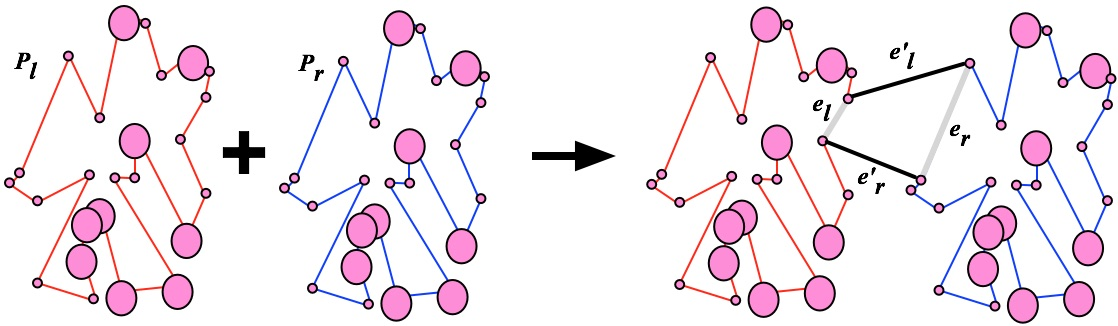
\includegraphics[width=6in]{./design/media-dc/etsp-merge.jpg}
\end{center}
%\newcommand{\norm}[1]{\ensuremath{\left\Vert #1 \right\Vert}}
To choose which swap to make, we consider all pairs of edges of
the recursive solutions consisting of one edge $e_\ell = (u_\ell,v_\ell)$ from
the left and one edge $e_r = (u_r,v_r)$ from the right and determine which
pair minimizes the increase in the following
cost: 
\[
\cdvar{swapCost}((u_\ell,v_\ell), (u_r,v_r)) =
\norm{u_\ell-v_r} + \norm{u_r-v_\ell} - \norm{u_\ell-v_\ell} -
\norm{u_r-v_r}
\] where $\norm{u-v}$ is the Euclidean distance between
points $u$ and $v$.

\end{gram}



\begin{algorithm}[Divide-and-Conquer eTSP]

By refining the intuition describe above, we arrive at a
divide-and-conquer algorithm for solving eTPS, whose pseudo-code is
shown below.

\[
\begin{array}{l}
\cdvar{eTSP}~(P) =
\\
~~~~\cd{if}~|P| < 2~\cd{then}
\\
~~~~~~~~\cd{raise}~\cdvar{TooSmall}
\\
~~~~\cd{else if}~|P| = 2~\cd{then}
\\
~~~~~~~~\cseq{(P[0],P[1]),(P[1],P[0])}
\\
~~~~\cd{else}
\\
~~~~~~~~\cd{let}
\\
~~~~~~~~~~~~(P_\ell, P_r) = \cdvar{split}~P~\cd{along the longest dimension}
\\
~~~~~~~~~~~~(L, R) = (\cdvar{eTSP}~P_\ell) \cpar{} (\cdvar{eTSP}~P_r)
\\
~~~~~~~~~~~~(c,(e,e')) = \cdvar{minVal}_{\cdvar{first}} \cset{(\cdvar{swapCost}(e,e'),(e,e')) : e \in L, e' \in R}
\\
~~~~~~~~\cd{in}
\\
~~~~~~~~~~~~~~~~\cdvar{swapEdges}~(\cdvar{append}~(L,R),e,e')
\\
~~~~~~~~\cd{end}
\end{array}
\]

The function $\cdvar{minVal}_{\cdvar{first}}$ uses the first value of
the pairs to find the minimum, and returns the (first) pair with that minimum. The function
$\cdvar{swapEdges}(E,e,e')$ finds the edges $e$ and $e'$ in $E$ and
swaps the endpoints. As there are two ways to swap, it picks the
cheaper one.
\end{algorithm}

\begin{remark} 
This heuristic divide-and-conquer algorithm is known to work well in
practice.
\end{remark}



\begin{gram}[Cost Analysis]

Let's analyze the cost of this algorithm in terms of work and
span.  
%
We have
\begin{align*}
  W(n) & = 2W(n/2) + O(n^2)\\
  S(n) & =  S(n/2) + O(\log n)
\end{align*}
%

We have already seen the recurrence $S(n) = S(n/2) + O(\log n)$, which solves
to $O(\log^2 n).$  Here we'll focus on solving the work recurrence.  % Let's try
% the tree method first.


% TODO \ref{} the theorem should be moved to recurrences.
To solve the recurrence, we apply a 
%
\href{thm:analysis::recurrences::linear-plus}{theorem  proven earlier},
%
and obtain 
\[
W(n) = O(n^2).
\]
\end{gram}

\begin{gram}[Strengthening]
In applications of divide-and-conquer technique that we have consider so far in this chapter, we divide a problem instance into instances of the same problem.
%
For example, in sorting, we divide the original instance into  smaller instances of the sorting problem.
%
Sometimes, it is not possible to apply this approach to solve a given problem, because solving the same problem on smaller instances does not provide enough information to solve the original problem.
%
Instead, we will need to gather more information
when solving the smaller instances to solve the original problem. 
%
In this case, we can \defn{strengthen} the original problem by requiring information in addition to the information required by the original problem.
%
For example, we might strengthen the sorting problem to return to us not just the sorted sequence but also a histogram of all the elements that count the number of occurrences for each element.
%% If you have seen the approach of strengthening an inductive hypothesis
%% in a proof by induction, it is very much an analogous idea.
%% Strengthening involves defining a problem that solves more than what
%% you ultimately need, but makes it easier or even possible to use
%% solutions of subproblems to solve the larger problem.
\end{gram}

\begin{teachnote}
Question:
You have recently seen an instance of strengthening when solving
a problem with divide and conquer. Can you think of the problem and
how you used strengthening?

In the recitation you looked at how to solve the Parenthesis Matching
problem by defining a version of the problem that returns the number
of unmatched parentheses on the right and left.  This is a stronger
problem than the original, since the original is the special case when
both these values are zero (no unmatched right or left parentheses).
This modification was necessary to make divide-and-conquer work---if
the problem is not strengthened, it is not possible to combine the
results from the two recursive calls (which tell you only whether the
two halves are matched or not) to conclude that the full string is
matched.  This is because there can be an unmatched open parenthesis
on one side that matches a close parenthesis on the other.
\end{teachnote}

\section{Divide and Conquer with Reduce}
\label{sec:design::dc::with-reduce}

\begin{gram}
Many divide-and-conquer algorithms have the following structure, where
$\cdvar{emptyVal}$, $\cdvar{base}$, and $\cdvar{myCombine}$ span for algorithm
specific values.

\[
\begin{array}{l}
\cdvar{myDC}~a =
\\ 
~~~~\cd{if}~|a| = 0 ~\cd{then}
\\
~~~~~~~~\cdvar{emptyVal}
\\
~~~~~~~~\cd{else if}~|a| = 1 ~\cd{then}
\\
~~~~~~~~~~~~\cdvar{base}(a[0])
\\
~~~~~~~~\cd{else}
\\
~~~~~~~~~~~~\cd{let}~(l,r) = \cdvar{splitMid}~a~\cd{in}
\\
~~~~~~~~~~~~~~~~(l',r') = (\cdvar{myDC}~l~\cpar{}~\cdvar{myDC}~r)
\\
~~~~~~~~~~~~\cd{in}
\\
~~~~~~~~~~~~~~~~\cdvar{myCombine}~(l', r')
\\
~~~~~~~~~~~~\cd{end}
\end{array}
\]

Algorithms that fit this pattern can be implemented in one line using
the sequence $\cdvar{reduce}$ function.
%
Turning a divide-and-conquer algorithm into a reduce-based solution is
as simple as invoking $\cdvar{reduce}$ with the following parameters
\[
\cdvar{reduce}~\cdvar{myCombine}~\cdvar{emptyVal}~(\cdvar{map}~\cdvar{base}~a).
\]
\end{gram}

\begin{important}
This pattern does not work in general for divide-and-conquer
algorithms.  In particular, it does not work for algorithms that do
more than an simple split that partitions their input in two parts in
the middle.  
%
For example, it cannot be used for implementing the quick-sort
algorithm, because the divide step partitions the data with respect to
a pivot.  
%
This step requires picking a pivot, and then filtering the
data into elements less than, equal, and greater than the pivot.  
%
It also does not work for divide-and-conquer algorithms that split
more than two ways, or make more than two recursive calls.
\end{important}

